\chapter{认知逻辑与共同知识}\label{chap:epistemic-logic}

\begingroup
\newcommand{\pref}{Chapters/epistemic-logic/figures}

\section{“泥泞的孩童”谜题}
{“泥泞的孩童”}
\begin{itemize}
    \item 有$n$个孩子在玩泥巴,他们互相泼泥巴.
    \item 母亲告诉孩子们,如果他们脸上沾上了泥巴,会受到严厉的惩罚.
    \item 孩子们不能看到自己的脸,但是可以看到其他所有人的脸.
    \item 所有孩子都希望保持自己的脸干净,但是弄脏别人的脸.
\end{itemize}

{“泥泞的孩童”}
\begin{itemize}
    \item 此时,孩子的父亲出现了,于是,孩子们停止泼泥巴.
    \item 孩子们互相不说话.
    \item 父亲看到了$k$($k\geq 1$)个人脸上有泥巴,于是宣布:
\end{itemize}
    \begin{center}
        “你们至少有一个人脸上沾了泥巴.”
    \end{center}


{“泥泞的孩童”}
\begin{itemize}
    \item 之后,父亲会公开地问若干轮如下问题:
\end{itemize}
\begin{center}
    “你们知道自己脸上有泥巴了吗?”
\end{center}
\begin{itemize}
    \item 孩子们回答“知道”或者“不知道”.
    \item 假设孩子们观察力敏锐、聪慧且诚实,并且每一轮他们都同时回答.
    \item 接下来会发生什么?
\end{itemize}


{“泥泞的孩童”:谜底}
\begin{itemize}
    \item 假设有$k$个孩子脸上有泥巴.
    \item 谜底:在前$k-1$轮中,所有孩子都会说“不知道”,在第$k$轮中,所有脸上有泥巴的孩子都会说“知道”.
    \item “证明”:对$k$归纳.
\end{itemize}


{“泥泞的孩童”:谜底}
\begin{itemize}
    \item 当$k=1$时,脸上沾满泥巴的孩子看到其他人都没有泥巴. 
    \item 既然他知道至少有一个孩子的脸上有泥巴,他就能推出那个人肯定是他自己. 
\end{itemize}



{“泥泞的孩童”:谜底}
\begin{itemize}
    \item 现在假设$k=2$,脸上沾满泥巴的孩子是$a$和$b$. 
    \item 一开始,因为他们分别看到了对方的脸上有泥巴,所以他们每个人都回答“不知道”. 
    \item 但是,当$b$回答“不知道”时,$a$意识到他自己肯定是脸上有泥巴的那个孩子,否则$b$就会在第一轮中知道泥巴在他的脸上,并回答“知道”. 因此,$a$在第二轮回答“知道”. 
    \item $b$也会通过同样的推理得出相同的结论. 
\end{itemize}


{“泥泞的孩童”:谜底}
\begin{itemize}
    \item 现在假设$k=3$,脸上沾满泥巴的孩子分别是$a$,$b$和$c$. 
    \item 孩子$a$的论证如下. 
    \begin{itemize}
        \item 假设我没有泥巴落在脸上. 
        \item 根据$k=2$的情况,$b$和$c$在第二轮都会回答“是”. 
        \item 他们没有这样做,我意识到假设是错误的,我的脸上也有泥巴.
        \item 因此在第三轮我会回答“知道”. 
    \end{itemize}
    \item $b$和$c$的论证也是类似的.
    \item $k=3$的论证具有一般性,所以归纳假设成立.
\end{itemize}


{“蓝眼睛红眼睛”谜题}
\begin{itemize}
    \item “泥泞的孩童”还有其他流行的陈述方式,比如“蓝眼睛红眼睛”.
    \item 一个岛上有100个人,其中有5个红眼睛,95个蓝眼睛.
    \item 这个岛有三个奇怪的宗教规则.
    \begin{enumerate}
        \item 他们不能照镜子,不能看自己眼睛的颜色. 
        \item 他们不能告诉别人对方的眼睛是什么颜色. 
        \item 一旦有人知道了自己的眼睛是红色,他就必须在当天夜里自杀.
    \end{enumerate}
    \item 岛民是不知道具体有几个红眼睛. 
\end{itemize}


{“蓝眼睛红眼睛”谜题}
\begin{itemize}
    \item 某天,有个旅行者到了这个岛上. 
    \item 由于不知道这里的规矩,所以他在和全岛人一起狂欢的时候,一不留神说了一句话:
    \begin{center}
        “你们这里有红眼睛的人. ”
    \end{center}
    \item 假设这个岛上的人足够聪明,每个人都可以做出缜密的逻辑推理. 
    \item 请问这个岛上将会发生什么?
\end{itemize}


{为什么会这样?}
\begin{itemize}
    \item 如果$k>1$,那么所有人都知道$p$:“至少有一个人脸上有泥巴”.
    \item 那么父亲说这句话的意义是什么?
    \item 如果父亲没有说$p$,那么会发生什么?
    \item 无论父亲问多少轮,所有孩子都只会回答“不知道”!(为什么)% HW
    \item 因此,父亲公开说了$p$,这是谜题的关键.
\end{itemize}


{$k=2$的情况分析}
\begin{itemize}
    \item 假设$k=2$,脸上沾满泥巴的孩子是$a$和$b$. 
    \item 在父亲宣布$p$之前,$a$和$b$都知道$p$.
    \item 然而,他们并不知道对方知道$p$. $a$可能会有两种想法:
    \begin{itemize}
        \item 我的脸上有泥巴,所以$b$知道$p$.
        \item 我的脸上没有泥巴,$b$是唯一一个有泥巴的,所以$b$不知道$p$.
    \end{itemize}
    \item 当父亲宣布$p$之后,$a$知道了$b$知道$p$.
    \item 当第一轮$b$回答“不知道”之后,$a$可以用“$b$知道$p$”这一知识推出自己脸上有泥巴.
\end{itemize}


{$k=3$的情况分析}
\begin{itemize}
    \item 假设$k=3$,脸上沾满泥巴的孩子是$a$,$b$和$c$. 
    \item 在父亲宣布$p$之前,$a$,$b$和$c$不仅知道$p$,而且知道彼此知道$p$.
    \begin{itemize}
        \item 以$a$的视角看,$b$能看到$c$脸上有泥巴,所以$a$知道$b$知道$p$.
    \end{itemize}
    \item 但是,$a$,$b$,$c$都不知道所有人知道所有人知道$p$!
\end{itemize}


{父亲宣布$p$的意义}
\begin{itemize}
    \item 用$E^m p$表示所有人知道所有人知道……所有人知道($m$次)$p$.
    \item 在一般情况下,父亲没有宣布$p$之前,$E^k p$并不成立.
    \item 父亲宣布了$p$之后,对任意$m\geq 1$,$E^m p$都成立!
    \item 因此,父亲宣布$p$带来了\emph{共同知识}(common knowledge).
    \item 有了共同知识,这一谜题就可以按照我们所讨论的方式进行下去.
\end{itemize}


{共同知识假设}
\begin{itemize}
    \item 我们曾经假设过所有人“观察力敏锐、聪慧且诚实”.
    \item 然而,这一假设并不足够.
    \item 我们必须假设所有人都知道所有人“观察力敏锐、聪慧且诚实”,所有人都知道所有人都知道所有人“观察力敏锐、聪慧且诚实”,……
    \item 换言之,我们需要假设“所有人观察力敏锐、聪慧且诚实”是共同知识.
    \item 假设还是只有两个孩子$a,b$脸上有泥巴.
    \item 假如$a$不知道$b$是诚实的,即便$b$回答了“不知道”,$a$也无法从$b$的回答中得到任何额外的知识!
\end{itemize}


{共同知识假设}
\begin{itemize}
    \item 除了假设“所有人观察力敏锐、聪慧且诚实”是共同知识,我们还需要假设以下陈述是共同知识:
    \begin{itemize}
        \item 每个人都能看到所有除自己外的人.
        \item 每个人都听到了父亲说的话.
        \item 父亲是诚实的.
        \item 每个人都在每一轮进行了充分的推理.
        \item ……
    \end{itemize}
    \item 任何假设的破坏都会导致之前的讨论失效.
    \item 那么,为什么父亲宣布$p$就可以让$p$变成共同知识呢?
\end{itemize}


{共同知识的产生}
\begin{itemize}
    \item 所有人都\emph{听到}父亲说$p$并不能产生共同知识.
    \item 假如父亲只是对每一个孩子单独宣布$p$.
    \begin{itemize}
        \item 所有人并不知道所有人都知道$p$,因而仅仅可以做到$E p$.
    \end{itemize}
    \item 那么,所有人都\emph{知道}所有人听到父亲说$p$会如何呢?
    \item 进一步假设每个孩子给每一个孩子都安装了窃听器,每个人都能够偷听每个人与父亲的谈话内容.
    \begin{itemize}
        \item 所有人并不知道所有人都知道所有人都知道$p$,因而仅仅有$E^2 p$.
    \end{itemize}
    \item 因此,父亲宣布$p$会产生共同知识的核心原因是“公开宣布”,此时对每一个$m$都有$E^m p$.
\end{itemize}


{启示}
\begin{itemize}
    \item “泥泞的孩童”谜题足以表明,关于“知道”的讨论远比想象的复杂.
    \item 关于“知道”(know)和知识(knowledge)的研究在哲学中划归为\emph{知识论}(epistemology).
    \item 接下来,我们将使用模态逻辑来形式化关于“知道”和知识的讨论,这被称之为\emph{认知逻辑}(epistemic logic).
\end{itemize}


\section{认知逻辑的基本模型与性质}
{命题认知逻辑}
\begin{itemize}
    \item 假设有$n$个人,分别叫$1,2,\dots,n$.
    \item 基本命题集为$\mathbf P$,用字母$p,q,r,\dots$表示基本命题.
    \begin{itemize}
        \item 例如,$p$表示“孩子$1$的脸上有泥巴”.
    \end{itemize}
    \item 回忆:逻辑框架是一个三元组(语言,模型,语义).
    \item 命题认知逻辑的的三元组是:
    \begin{itemize}
        \item 语言$L_n$:命题逻辑加上模态算子$K_i,i=1,\dots,n$.
        \item 模型$\mathcal M,w$:Kripke模型
        \item 语义$\vDash$:可能世界语义
    \end{itemize}
\end{itemize}

{命题认知逻辑}
\begin{itemize}
    \item 模态公式$K_i\phi$被读作“$i$知道$\phi$”.
    \item 从语义来说,$K_i$是$\Box$算子,即我知道$\phi$意味着在我认为的所有可能世界中$\phi$都是真的.
    \begin{itemize}
        \item $\mathcal M,w\vDash K_i\phi$当且仅当对任意$v$,如果$w\to_i v$,那么$\mathcal M,v\vDash\phi$.
    \end{itemize}
    \item 模态公式的真值有两个层面:
    \begin{itemize}
        \item 在点模型上可满足:$\mathcal M,w\vDash\phi$.
        \item 在框架上有效:$\mathcal F\vDash\phi$.
    \end{itemize}
\end{itemize}

{例子}
\begin{itemize}
    \item 虽然我们没有定义$K_i$的对偶算子,但是$K_i$的对偶相当于$\Diamond$算子.
    \item $\neg K_i\neg\phi$表示的意思是“$i$不知道$\phi$不是真的”,因此$i$会考虑$\phi$可能是真的. 当然,这也意味着$i$会考虑$\neg\phi$也可能是真的.
    \item “我不知道上帝存在” vs. “我知道上帝不存在”.
    \begin{itemize}
        \item $\neg Kp$ vs. $K\neg p$.
        \item 显然,前者是更弱的一种表述,因此$\neg K$和$K\neg$的含义完全不同.
    \end{itemize}
\end{itemize}


{例子}
\begin{itemize}
    \item $K_1K_2p\wedge \neg K_2K_1K_2 p$.
    \begin{itemize}
        \item $1$知道$2$知道$p$,但是$2$并不知道$1$知道$2$知道$p$.
    \end{itemize}
    \item $\neg K_i p\to K_i(\neg K_i p)$.
    \begin{itemize}
        \item 如果我不知道$p$,那么我知道我不知道$p$.
    \end{itemize}
    \item $K_i(p\wedge\neg K_i p)$.
    \begin{itemize}
        \item 我知道如下的陈述:$p$是真的,且我不知道$p$.
        \item 一种类似的写法是,$K_ip\wedge K_i\neg K_ip$.
        \item 我知道$p$,但是我又知道我不知道$p$.
    \end{itemize}
\end{itemize}


{Kripke模型的限制}
\begin{itemize}
    \item 模态算子$K_i$有特殊的性质,这要求我们对$K_i$对应的关系$R_i$也有额外的要求.
    \item 我们要求每一个$R_i$都是等价关系$\sim_i$:
    \begin{itemize}
        \item 自反:$\forall x\, x\sim_ix$.
        \item 传递:$\forall x,y,z(x\sim_iy\wedge y\sim_iz)\to x\sim_iz$.
        \item 对称:$\forall x,y(x \sim_i y\leftrightarrow y\sim_ix)$.
    \end{itemize}
    \item 从可能世界的角度来说,这一要求就是说对$i$来说,她所认为可能的世界之间都是不可区分的.
\end{itemize}

{算子$K_i$的公理}
\begin{itemize}
    \item 从模态可定义性的角度来说,$R_i$的特殊性质会对应$K_i$特殊的公式.
    \item 这些公式就可以被看成关于“知道”的公理(模式)或推导规则.
    \item 承认某一条公理(模式)或推导规则就必须承认可能世界具有某一种性质,反之亦然.
\end{itemize}

{分配公理}
\begin{itemize}
    \item \emph{分配公理}(distribution axiom):$\vDash (K_i(\phi\to\psi)\wedge K_i\phi)\to K_i\psi$.
    \item 有效性验证.
    \begin{itemize}
        \item 假设$\mathcal M,w\vDash K_i(\phi\to\psi)$且$\mathcal M,w\vDash K_i \phi$.
        \item 于是,对所有$R_i$后继$v$都有$\mathcal M,v\vDash\phi\to\psi$和$\mathcal M,v\vDash\phi$,因而$\mathcal M,v\vDash\psi$.
        \item 根据定义,$\mathcal M,w\vDash K_i\psi$,因而对所有$\mathcal F$,分配公理有效.
    \end{itemize}
    \item 类比:演绎推理的肯定前件(Modus ponens,MP)推导规则.
    \item 分配公理意味着拥有知识的个体可以对自己的知识做任意的演绎推理,因而假设个体是\emph{逻辑全知的}(logically omniscient).
\end{itemize}

{知识泛化规则}
\begin{itemize}
    \item \emph{知识泛化规则}(knowledge generalization rule):对所有$\mathcal F$,如果$\mathcal F\vDash\phi$,那么$\mathcal F\vDash K_i\phi$.
    \item 有效性验证.
    \begin{itemize}
        \item 假设$\mathcal F\vDash\phi$,这意味着对所有基于$\mathcal F$的点模型都有$\mathcal M,w\vDash\phi$.
        \item 因此,对任意$w$的$R_i$后继$v$,也有$\mathcal M,v\vDash\phi$.
        \item 所以也有$\mathcal M,w\vDash K_i\phi$成立,因而$\mathcal F\vDash K_i\phi$.
    \end{itemize}
    \item 类比:一阶逻辑推理的泛化规则.
    \item 前提成立的$\phi$是关于$\mathcal F$本身的性质(特别是关于知识),因此知识泛化规则意味着个体知道关于知识的一切性质.
    \begin{itemize}
        \item 其实更重要的是,知识的一切性质都是共同知识(练习).% HW
    \end{itemize}
\end{itemize}


{知识公理}
\begin{itemize}
    \item \emph{知识公理}(knowledge axiom)或\emph{真理公理}(truth axiom):$\vDash_H K_i\phi\to\phi$.
    \item 验证留作练习. % HW
    \item 知识公理意味着,$i$知道的命题一定是真的.
    \item 在知识论中,这一要求实际上反映了“拥有知识”需要付出努力、值得一定的奖励.
    \item 与此相对应地,\emph{信念}(belief)则是更加主观、随意的,因而并不具有真理性.
    \begin{itemize}
        \item 我考试挂了,但不知道我考试挂了.
        \item 我考试挂了,但我不相信我考试挂了.
    \end{itemize}
\end{itemize}

{内省公理}
\begin{itemize}
    \item \emph{正内省公理}(positive introspective axiom):$\vDash_H K_i\phi\to K_iK_i\phi$.
    \item \emph{负内省公理}(positive introspective axiom):$\vDash_H \neg K_i\phi\to K_i\neg K_i\phi$.
    \item 验证留作练习. % HW
    \item 这两条公理意味着个体会通过内省来知道自己的处境,特别是“我知道什么”和“我不知道什么”.
    \item 思考:(负)内省公理是否合理?
\end{itemize}

{其他公理}
\begin{itemize}
    \item 以上五条性质(四条公理+一条推导规则)加上MP形成的推理系统称为S5公理系统.
    \begin{itemize}
        \item 需要注意的是,这些公理其实都是公理模式,包含了无穷条公理.
    \end{itemize}
    \item 此外,从哲学的角度讨论,还有一些别的公理.
    \item \emph{一致性公理}(consistency axiom):$\vDash_H\neg K_i\bot$.
    \begin{itemize}
        \item 因此,个体不能够知道假的陈述,以此区别于信念.
    \end{itemize}
\end{itemize}

{公理与模型结构}
\begin{itemize}
    \item 我们基于框架类$H$给出了关于知识的公理.
    \item 反过来,公理对应什么样的框架结构呢?
    \item 我们总结如下表:
    \begin{table}[ht]
        \centering
       \begin{tabular}{cc}
\toprule 公理 &  $R_i$的性质 \\
\midrule $K_i \varphi \to \varphi$ & 自反性 \\
$K_i \varphi \to K_i K_i \varphi$ & 传递性 \\
$\neg K_i \varphi \to K_i \neg K_i \varphi$ & 欧氏性 \\
$\neg K_i\bot$  & 序列性\\
$\varphi \to K_i \neg K_i \neg \varphi$ & 对称性 \\
\bottomrule
\end{tabular}
    \end{table}
\end{itemize}


{公理与模型结构}
\begin{itemize}
    \item 欧氏性:$\forall x,y,z(xR_iy\wedge xR_iz\to yR_iz)$.
    \begin{itemize}
        \item 关系一定形成三角形.
    \end{itemize}
    \item 序列性:$\forall x\exists y\, xR_iy$.
    \begin{itemize}
        \item 所有点都有后继.
    \end{itemize}
    \item 以上验证都留作习题. % HW   
    \item 思考:从可能世界角度,$R_i$的这些性质有什么直观的含义?
    \item 思考:为什么有些公理没有对应的结构性质?(提示:注意观察一个公理/规则是否有$H$出现)
\end{itemize}


{公理与模型结构}
\begin{itemize}
    \item 可以看出来,以上关系其实并不是孤立的,我们有:
\begin{lemma} %HW
\begin{itemize}
    \item 如果$R_i$是自反和欧氏的,那么$R_i$是对称和传递的.
    \item 如果$R_i$是对称和传递的,那么$R_i$是欧氏的.
    \item 以下命题等价:
    \begin{itemize}
        \item $R_i$是自反、对称和传递的.
\item  $R_i$是对称、传递和序列的.
\item $R_i$是自反和欧氏的.
    \end{itemize}
\end{itemize}
\end{lemma}
\item 证明留作练习.
\end{itemize}


{引入共同知识算子}
\begin{itemize}
    \item 下面我们将认知逻辑语言加入共同知识算子和它的语义.
    \item 首先加入“所有人都知道”这个算子:$E\phi\leftrightarrow\bigwedge_i K_i\phi$.
    \item 记$E^k\phi$为$\underbrace{E\dots E}_k\phi$.
    \item 于是,共同知识算子$C$的语义定义为:
    \[\mathcal M,w\vDash C\phi\iff\mathcal M,w\vDash E^k\phi,\quad k=1,2,\dots\]
\end{itemize}


{模型含义}
\begin{itemize}
    \item 我们可以从图结构来理解共同知识算子.
    \item $\mathcal M,w\vDash E^k\phi$的含义是,从$w$出发走$k$步可到达的可能世界$v$上都有$\mathcal M,v\vDash \phi$.
    \item $\mathcal M,w\vDash C\phi$的含义则是,从$w$出发可到达的可能世界$v$上都有$\mathcal M,v\vDash \phi$.
\end{itemize}


{共同知识的公理}
\begin{itemize}
    \item 类似算子$K_i$,$C$也有它对应的公理和推导规则.
    \item \emph{不动点公理}(fixed-point axiom):$\vDash C\phi\leftrightarrow E(\phi\wedge C\phi)$.
    \begin{itemize}
        \item 共同知识是一个递归方程的(最小)解,这是一种不动点的视角.
    \end{itemize}
    \item \emph{归纳规则}(induction rule):如果$\mathcal F\vDash \phi\to E(\phi\wedge\psi)$,那么$\mathcal  F\vDash \phi\to C\psi$.
    \begin{itemize}
        \item 每个人都可以从真实中得到的知识,一定是共同知识.
    \end{itemize}
    \item 将S5公理系统中加入关于$E$和$C$的公理,我们就扩展了认知逻辑. 
    \item 因为$E$和$C$是用$K_i$定义的,因此他们本身并不会带来Kripke模型新的结构性质.
\end{itemize}


{“泥泞的孩童”再回顾}
\begin{itemize}
    \item 现在,我们可以形式化、严格讨论“泥泞的孩童”这一谜题了.
    \item 这一问题对应的逻辑语言是认知逻辑语言.
    \item 可能世界是$\{0,1\}^n$的元素$x=(x_1,\dots,x_n)$,$x_i=1$表示孩子
    $i$脸上有泥巴,$x_i=0$表示$i$脸上没有泥巴.
    \item 假设每个孩童$i$对应的$R_i$都是一个等价关系.
    \item 当我们如此假设时,每个孩子唯一不是共同知识的事情就是脸上泥巴的状态,其他的所有事情都被隐含在了共同知识之中.
\end{itemize}


{“泥泞的孩童”再回顾}
\begin{itemize}
    \item 原子命题$p_i$:孩子$i$脸上有泥巴,$p$:至少有一个孩子脸上有泥巴.
    \item 假设现在父亲还没有说出$p$.
    \item 对于孩子$i$,他的认知中只有两个可能世界:我的脸上有泥巴,或者我的脸上没有泥巴,其他对他来说都是确定的.
    \begin{itemize}
        \item $x R_i y$当且仅当$x_j=y_j$对任意$j\neq i$成立.
    \end{itemize}
    \item 因此,框架$\mathcal F$会对应一个$n$维超立方体.
\end{itemize}


{“泥泞的孩童”再回顾}
\begin{itemize}
    \item $n=3$的例子:
\end{itemize}
\begin{figure}[ht]
    \centering
    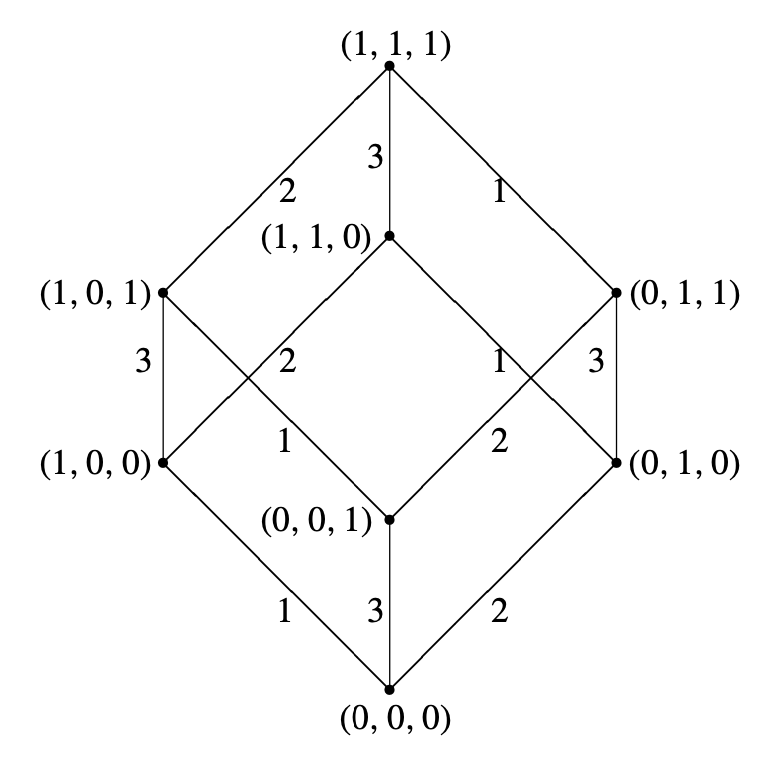
\includegraphics[scale=0.4]{\pref/cubic-example.png}
\end{figure}


{“泥泞的孩童”再回顾}
\begin{itemize}
    \item 从框架$\mathcal F$到模型$\mathcal M$,我们还需要确定赋值$V$.
    \item $w\in V(p_i)$当且仅当$w_i=1$.
    \item $w\in V(p)$当且仅当所有分量$w_j$不全为零.
    \item 从模型到点模型,我们还需要确定我们所处的可能世界,于是我们就可以讨论模态公式的可满足性.
    \item 例如:$\mathcal M,(1,0,1)\vDash Ep$,但是$\mathcal M,(1,0,1)\vDash \neg E^2p$.
\end{itemize}


{“泥泞的孩童”再回顾}
\begin{itemize}
    \item 假设现在父亲宣布了$p$,那么$\mathcal F$将会发生变化:
\end{itemize}
\begin{figure}[ht]
    \centering
    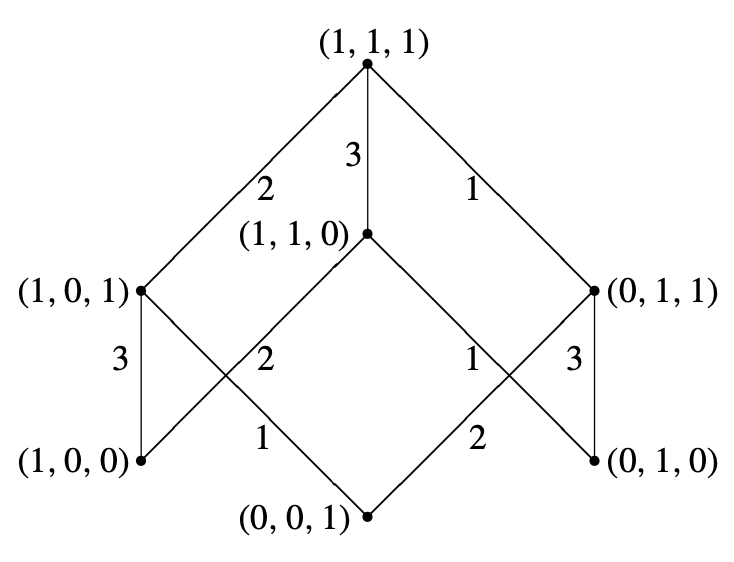
\includegraphics[scale=0.5]{\pref/cubic-example-after-father.png}
\end{figure}


{“泥泞的孩童”再回顾}
\begin{itemize}
    \item 在$i$眼中,只有两个可能世界,因此$i$回答“知道”意味着她能够确定只有一个世界;她回答不知道意味着还有两个可能世界.
    \item 假如现在是第一轮问答.
    \item 如果所有人都回答了“不知道”,考虑状态$s=(1,0,0,\dots)$.
    \item 如果真实世界是$s$,那么对于$1$来说,可能世界只有一个了,但是她却说“不知道”,说明真实世界不是$s$.
    \item 同理,所有那些只有一个$1$的可能世界都会被消掉.
    \item 因此,归纳可得,第$k$轮的时候,所有那些只有$k$个$1$的可能世界会被消掉. % HW:证明这个
\end{itemize}


{“泥泞的孩童”再回顾}
\begin{itemize}
    \item 如果父亲没有宣布$p$,那么$\mathcal M$是一个超立方体.
    \item 无论在任何轮,每一个孩子都会觉得两个可能世界,因此不会有任何可能世界被消掉!
    \item 因此,从结构上来说,父亲宣布$p$改变了每个孩子对应的$R_i$等价的可能世界,使得一些孩子可以确定自己所处的世界.
    \item 这一套方法可以将类似的智力谜题都用算法化的方式得到解答.
\end{itemize}


{基于事件的认知理论}
\begin{itemize}
    \item 如果我们限制Kripke模型中$R_i$为等价关系,那么认知逻辑还可以有另一种理解方式.
    \item 回忆:概率论(或者似然)理解世界的方式基于“事件”.
    \item 我们只能感知事件的发生与否,而不能具体知道是哪个样本点.
    \item 用事件的方式理解认知,得到的结构被称为\emph{Aumann结构}.
\end{itemize}


{Aumann结构}
\begin{itemize}
    \item 考虑全集$\Omega$,理解为样本空间.
    \item 事件$e\subseteq \Omega$是样本点的集合.
    \item 一次观测会落实在一个样本点$\omega$上.
    \item 事件$e$发生当且仅当$\omega\in e$.
    \item 在Kripke模型中,我们将$i$的知识刻画为了等价关系$R_i$.
    \item 在Aumann结构中,对每一个个体$i$,它的知识被刻画为$\Omega$的划分$\mathcal P_i=\{\Omega_j\}$,$\Omega_j$是$\Omega$的子集.
    \item $S_j$被称为$i$的\emph{信息集}(information sets),可以被理解为$i$能够感知到的最基本的事件.
\end{itemize}    


{Aumann结构}
\begin{itemize}
    \item $\mathcal P_i(\omega)$被定义为$\omega$所属于的那个信息集.
    \item 现在我们重新定义算子$K_i:2^\Omega\to 2^\Omega$为
    \[K_i(e):=\{\omega\in\Omega:\mathcal P_i(\omega)\subseteq e\}.\]
    \item $K_i(e)$定义了“个体$i$知道事件$e$”这一事件.
    \item 思想:将所有关于知识的讨论转化为关于事件的讨论.
\end{itemize}


{Aumann结构}
\begin{itemize}
    \item 类似地,可以定义算子$E:2^\Omega\to 2^\Omega$为:
    \[E(e)=\bigcap_{i=1}^n K_i(e).\]
    \item 定义共同知识算子$C:2^\Omega\to 2^\Omega$为:
    \[C(e)=\bigcap_{k=1}^\infty E^k(e).\]
\end{itemize}


{Kripke模型与Aumann结构的关系}
\begin{itemize}
    \item 我们再一次看到逻辑和集合的对应,我们总结如下表:
    \begin{table}[ht]
        \centering
        \begin{tabular}{cc}
        \toprule
             Kripke模型&Aumann结构  \\\midrule
             可能世界&样本点\\
             公式&事件\\
             原子命题&基本事件\\
             模态算子&集合-集合映射\\
             $i$的等价关系$R_i$&$i$的划分\\
             逻辑连接词&集合操作\\\bottomrule
        \end{tabular}
    \end{table}
\end{itemize}


{Kripke模型与Aumann结构的关系}
\begin{itemize}
    \item Kripke语义偏好逻辑,Aumann结构偏好(Bayes)概率论,因此用数学来研究知识论就有了两种风格,一种是计算机、逻辑、哲学的风格,另一种是经济学、信息论的风格.
    \item 但是,这两种对应关系完全取决于我们对知识的那些基本假设,所以如果这些假设被打破,那么这样的对应关系就不再成立!
    \item 下面我们分别用这两种风格来讨论共同知识的意义.
\end{itemize}


\section{对不一致达成一致}
{问题背景}
\begin{itemize}
    \item 本部分将用模态逻辑的方式来探讨达成一致与共同知识的关系.
    \item 最早由Aumann给出.
    \item 我们将要证明,对于有相同决策方式的两个个体来说,他们不可能对采取不同行动这件事具有共同知识.
    \item 典型故事:同样的AI之间会发生交易吗?
    \item 交易发生意味着买家和卖家有不一样的决策(一个买一个卖).
    \item 因此,如果两个人按照相同的规则来行事,那么不会有交易发生!
\end{itemize}
\begin{center}
    players cannot ``agree to disagree''.
\end{center}


{模型}
\begin{itemize}
    \item 假想一个含时的系统,有两个玩家1和2.
    \item 在任意时刻,每个玩家处于一个状态$s_i$之中.
    \item 每个玩家分别有一个自己的局部状态空间$S_i$.
    \item 整个系统的全局状态是$(s_1,s_2)\in S_1\times S_2=\mathcal G$.
    \item 时刻是离散的,用非负整数$m$表示,初始时刻是$0$.
    \item 系统的一次\emph{运行}(run)指的是函数$r:m\mapsto(s_1,s_2)$.
    \begin{itemize}
        \item 运行描述了系统每一时刻的全局状态.
    \end{itemize}
    \item \emph{系统}(system)$\mathcal R$指的是$\mathcal G$上所有可能运行的集合.
    \item 给定$r\in\mathcal R$,$(r,m)$被称为系统$\mathcal R$的一个点.
\end{itemize}


{模型}
\begin{itemize}
    \item 玩家处于某个状态的时候可以采取某种行动.
    \item 为了反映“玩家按照相同的规则行事”这件事,我们规定两个玩家的行动集都是$A$,并且这一集合不依赖于全局或局部的状态.
    \item 给定所有人的行动和一个全局状态,我们可以定义系统的\emph{转移函数}(transition function)为$\tau:A^2\times\mathcal G\to\mathcal G$.
    \begin{itemize}
        \item 因此,转移函数描述了所有人的行动如何导致系统从一个状态到另一个状态.
    \end{itemize}
\end{itemize}


{模型}
\begin{itemize}
    \item 如何描述“按照规则行事”?
    \item 我们用\emph{协议}(protocol)来描述这种概念.
    \item 玩家$i$的协议$P_i$是一个从局部状态$S_i$到行动集$A$的映射.
    \begin{itemize}
        \item 处于什么状态就做什么事.
    \end{itemize}
    \item 两个玩家的联合协议记为$P=(P_1,P_2)$.
\end{itemize}


{模型}
\begin{itemize}
    \item 一个联合协议要执行起来,还需要初始状态.
    \item 初始状态可能的集合记为$\mathcal G_0$.
    \item 给定初始状态集$\mathcal G_0$和转移函数$\tau$,我们就可以在系统上执行任何一种协议.
    \item 我们把元组$\gamma=(\mathcal G_0,\tau)$称为系统的\emph{上下文}(context).
\end{itemize}



{模型}
\begin{itemize}
    \item 给定上下文$\gamma=(\mathcal G_0,\tau)$和一个联合协议$P$,我们可以讨论$P$产生的所有可能运行.
    \item 一个运行$r$与$P$\emph{相容}(compatible)指的是
    \begin{itemize}
        \item $r(0)\in\mathcal G_0$.
        \item 对任意时刻$m$,如果$r(m)=(s_1,s_2)$,那么$r(m+1)=\tau(P(s_1),P(s_2))(s_1,s_2)$.
    \end{itemize}
    \item 换言之,$r$是从跟某个可能的初始状态开始执行协议产生的运行.
    \item 一个系统$\mathcal R$表示了上下文$\gamma$和联合协议$P$,指的是所有$r\in\mathcal R$都与$P$相容. 这样的系统我们用记号$\mathcal R^{rep}(P,\gamma)$来表示.
\end{itemize}




{模型}
\begin{itemize}
    \item 接下来我们引入Kripke模型.
    \item Kripke模型的点是系统的点.
    \item 设原子命题集$\mathbf P$,它的元素是$perf_i(a)$,表示玩家$i$采取行动$a$.
    \item 接下来我们定义赋值函数$V$.
    \item 从$\mathbf P$的定义来看,赋值应该只依赖状态,而不依赖时间,所以我们赋值函数实际上需要分两步来定义:
    \begin{itemize}
        \item 定义$V$为从$\mathbf P$到全局状态集合的映射,
        \item 然后再扩展为到系统点集合的映射:$(r,m)\in V(p)\iff r(m)\in V(p)$.
    \end{itemize}
    \item 第一步定义如下:状态$s\in V(perf_i(a))$当且仅当在状态$s$玩家$i$采取过行动$a$.
\end{itemize}


{模型}
\begin{itemize}
    \item 然后我们引入知识算子$K_i$的语义.
    \item 同样,我们假设$K_i$对应的是等价关系$\sim_i$.
    \item 玩家$i$只能区分自己的局部状态$s_i$,他执行协议时,只有状态,没有时间的概念.
    \item 因此我们定义$(r,m)\sim_i (r',m')\iff r(m)_i=r'(m')_i$.
    \item 从Aumann结构来说,每一个局部状态$s_i$对应了一个信息集
    \[IS_i(s_i,\mathcal R)=\{(r,m):r\in\mathcal R,r(m)=s_i\}.\]
    \item 这样,我们就得到了Kripke点模型$\mathcal M,(r,m)$.
    \item $K_i$的语义按照基本认知逻辑定义即可.
\end{itemize}


{模型}
\begin{itemize}
    \item 接下来,我们引入关于时间的模态算子.
    \item 特别地,我们只引入算子$X$,表示“下一时刻”.
    \item 它的语义定义为
    \[\mathcal M,(r,m)\vDash X\phi\iff\mathcal M,(r,m+1)\vDash\phi.\]
    \item 有了算子$X$,我们可以用公式表达“将要采取行动”:
    \[act_i(a)=\neg perf_i(a)\wedge X perf_i(a).\]
\end{itemize}



{模型}
\begin{itemize}
    \item 接下来,我们定义关于Kripke模型的\emph{决策函数}(decision function),用它来在点模型的角度讨论协议的执行.
    \item 设Kripke模型的点集为$S$.
    \item 玩家$i$的决策函数$D$是从$S$的某些子集到行动集$A$的映射.
    \begin{itemize}
        \item 我们没有写决策函数的下标,表明两个玩家采取了相同的决策策略.
    \end{itemize}
    \item 决策函数描述的是:知道什么样的信息,就采取什么样的行动.
    \begin{itemize}
        \item 回忆Aumann结构,$S$的子集是事件.
    \end{itemize}
\end{itemize}


{模型}
\begin{itemize}
    \item 我们要求协议$P_i$和决策函数$D$是相容的,也就是决策函数在某个信息集上采取的行动恰好是这个协议在该状态要执行的行动:
    \[P_i(s_i)=D(IS_i(s_i,\mathcal R)),\forall s_i\in S_i.\]
    \item 反过来说,联合协议$P$在上下文$\gamma$中\emph{实现}(implement)了决策函数$D$,如果对所有$i$,$P_i$与$D$在系统$\mathcal R^{rep}(P,\gamma)$中是相容的.
\end{itemize}


{模型}
\begin{itemize}
    \item 协议和决策函数是两个非常容易混淆的概念,尽管他们有密切联系.
    \item 直观来说,协议就是处于什么局部状态采取什么行动,这并不涉及知识的内容.
    \item 而决策函数指的是,知道什么信息就采取什么行动,这完全是知识的内容.
    \item 在我们的背景下,
    \[\text{知道的信息}=\text{处于的局部状态}.\]
    \item 因此二者其实是从不同角度描述同一个概念.
\end{itemize}


{模型}
\begin{itemize}
    \item 我们对决策函数$D$有一个额外的技术要求,我们要求$D$是并-一致的(union-consistent).
    \item 具体来说,给定$S$一列互不相交的子集$T_1,\dots,T_k$,每一个都有$D(T_i)=a$,那么我们要求$D(\cup_i T_i)=a$.
    \begin{itemize}
        \item 假设我的决策函数是这样描述的:如果今天下雨,并且今天星期四,那么我会去KFC疯狂星期四;如果今天不下雨,并且今天星期四,那么我会去KFC疯狂星期四.
        \item 那么,我的决策还应该有:虽然我不知道今天下不下雨,但是如果今天是星期四,那么我会去KFC疯狂星期四.
    \end{itemize}
    \item 性质:任何联合协议都可以从某个并-一致的决策函数产生.
\end{itemize}


{模型}
\begin{itemize}
    \item 我们现在回顾一下这个模型.
    \item 两个玩家处于同一个系统中.
    \item 每个玩家可能知道不同的东西(局部状态空间不同,信息集不同).
    \item 但是他们的行动集相同、决策函数相同.
    \item 决策函数要求是并-一致的,由某个联合协议实现.
    \item 给定可能的初始状态和系统的转移函数(上下文),系统可以产生一系列可能的运行.
\end{itemize}


{达成一致定理}
\begin{theorem}[Aumann,达成一致定理,Agreement theorem]
给定联合协议$P$,上下文$\gamma$,由此产生Kripke框架$\mathcal F$. 设$a,b\in A$是两个不同的行动,如果在上下文$\gamma$中$P$实现了某个并-一致决策函数,那么
\[\mathcal F\vDash\neg C(act_1(a)\wedge act_2(b)).\]
\end{theorem}
\begin{itemize}
    \item 如果两个玩家选择了同样的并-一致决策函数,那么他们不可能对“我们采取不同行动”这件事形成共同知识.
    \item 他们不可能对不一致达成一致(agree to disagree).
\end{itemize}


{达成一致定理:证明}
\begin{itemize}
    \item 用反证法. 假设某个基于$\mathcal F$的点模型$\mathcal M,(r,m)$使得
    \[\mathcal M,(r,m)\vDash C(act_1(a)\wedge act_2(b)).\]
    \item 我们证明$a=b$.
    \item 思路:
    \begin{itemize}
        \item 共同知识对应了从$(r,m)$出发可到达的状态集$S'$的性质.
        \item 从玩家1的视角来看,她在$S'$所关联的信息集上都要采取行动$a$,根据并-一致性,应该有$D(S')=a$.
        \item 从玩家2来看同理,因此也应该有$D(S')=b$.
        \item 因此$a=b$.
    \end{itemize}
\end{itemize}


{达成一致定理:证明}
\begin{itemize}
    \item 假设$S'$是从$(r,m)$出发,通过关系$\sim_1$或$\sim_2$可到达的点集.
    \item 取一个点$(r',m')\in S'$,设$r'(m')_1=s_1'$.
    \item 假设$(r'',m'')\sim_1(r',m')$,那么$(r'',m'')\in S'$.
    \item 因此,$IS_1(s_1',\mathcal R)\subseteq S'$.
    \item 当$s_1'$取遍$S_1$,根据信息集的性质,$S'$是$IS_1(s_1',\mathcal R)$的不交并.
\end{itemize}


{达成一致定理:证明}
\begin{itemize}
    \item 因为$\mathcal M,(r,m)\vDash C(act_1(a))$,所以有$\mathcal M,(r',m')\vDash act_1(a)$.
    \item 这一公式意味着$P_1(s_1')=a$.
    \item 根据$P$和$D$的关系,这等价于$D(IS_1(s_1',\mathcal R))=a$.
    \item 因为这件事对任意$s_1'$都成立,根据$D$的并-一致性,$D(S')=a$.
    \item 同理,从玩家2的角度来说$D(S')=b$.
    \item 因此$a=b$.
\end{itemize}


{达成一致定理:拓展}
\begin{itemize}
    \item 我们的定理是对于确定性的协议证明的.
    \item 然而,一个协议可能是非确定的,也就是在一个状态可能会有多种行动的选择,比如选择带有随机性.
    \item 这个时候,达成一致定理依然成立,但是我们需要恰当地定义Kripke模型、决策函数以适应非确定性的协议.
    \item 当协议具有非确定性时,我们可以用这一模型来理解带有先验知识(分布)、风险或者不确定性下的达成一致定理.
    \begin{itemize}
        \item 只要协议能够对应一个并-一致的决策函数,结论都有效.
    \end{itemize}
\end{itemize}


\section{Rubinstein电子邮件博弈}
{Rubinstein电子邮件博弈}
\begin{itemize}
    \item 接下来我们使用Bayes概率论来说明在二人静态博弈中,共同知识对到底实现哪一个Nash均衡非常关键.
    \item 此时,知道一件事与否被赋予了不确定性的含义:我确定或不确定某件事发生.
\end{itemize}

{Decision Letter on the``E-Mail Game'', AER, 1989}
\begin{center}
    \begin{minipage}[c]{0.8\textwidth}
\footnotesize
\hfill 30 March, 1988

Dear Ariel,

\hfill

Please find enclosed two thoughtful reports (actually, one is thoughtful; the other one is just silly) on your stimulating paper ``the e-mail game'', which you submitted for publication in the AER. As you will see, it's quite impossible to understand what they're trying to say, or what their final recommendation is.

Now, I didn't feel like reading your paper myself. You seem like a nice guy, the title of the paper is catchy, and people say you write pretty good papers, so I decided to accept your paper for publication. You also won a free ticket to a Broadway musical of your choice.

\hfill

Sincerely yours, 

The Editor
\end{minipage}
\end{center}


{Rubinstein电子邮件博弈}
\begin{table}[ht]
    \centering
\begin{tabular}{c|cc}
&$A$ & $B$ \\
\hline
$A$ & $(0, 0)$ & $(-10, 1)$ \\
$B$ & $(1, -10)$ & $(8, 8)$ \\
\end{tabular}
\qquad
\begin{tabular}{c|cc}
&$A$ & $B$ \\
\hline
$A$ & $(8, 8)$ & $(-10, 1)$ \\
$B$ & $(1, -10)$ & $(0, 0)$ \\
\end{tabular}
\end{table}
\begin{itemize}
\item 两个玩家和两个可能的矩阵.
\item 在左边的矩阵中:
\begin{itemize}
\item $(B,B)$是唯一的Nash均衡.
\end{itemize}
\item 在右边的矩阵中:
\begin{itemize}
\item 这是一个协作博弈.
\item 多个Nash均衡:$(A,A)$和$(B,B)$.
\item 观察:$(A,A)$给出比$(B,B)$更高的收益,但行动$A$比$B$更有风险.
\end{itemize}
\end{itemize}


{Rubinstein电子邮件博弈}
\begin{table}[ht]
    \centering
\begin{tabular}{c|cc}
&$A$ & $B$ \\
\hline
$A$ & $(0, 0)$ & $(-10, 1)$ \\
$B$ & $(1, -10)$ & $(8, 8)$ \\
\end{tabular}
\qquad
\begin{tabular}{c|cc}
&$A$ & $B$ \\
\hline
$A$ & $(8, 8)$ & $(-10, 1)$ \\
$B$ & $(1, -10)$ & $(0, 0)$ \\
\end{tabular}
\end{table}
\begin{itemize}
\item 左边矩阵被选择的概率是$p>1/2$.
\item 玩家1知道真实的矩阵,而玩家2不知道.
\item 如果选择了右边矩阵,玩家1会给玩家2发送一条消息.
\end{itemize}



{Rubinstein电子邮件博弈}
\begin{table}[ht]
    \centering
\begin{tabular}{c|cc}
&$A$ & $B$ \\
\hline
$A$ & $(0, 0)$ & $(-10, 1)$ \\
$B$ & $(1, -10)$ & $(8, 8)$ \\
\end{tabular}
\qquad
\begin{tabular}{c|cc}
&$A$ & $B$ \\
\hline
$A$ & $(8, 8)$ & $(-10, 1)$ \\
$B$ & $(1, -10)$ & $(0, 0)$ \\
\end{tabular}
\end{table}
\begin{itemize}
\item 如果玩家2收到了消息,她会回复.  
\item 如果玩家1收到了回复,她会发送第二条消息来确认她收到了玩家2的回复.  
\item 以此类推.  
\end{itemize}


{Rubinstein电子邮件博弈}
\begin{table}[ht]
    \centering
\begin{tabular}{c|cc}
&$A$ & $B$ \\
\hline
$A$ & $(0, 0)$ & $(-10, 1)$ \\
$B$ & $(1, -10)$ & $(8, 8)$ \\
\end{tabular}
\qquad
\begin{tabular}{c|cc}
&$A$ & $B$ \\
\hline
$A$ & $(8, 8)$ & $(-10, 1)$ \\
$B$ & $(1, -10)$ & $(0, 0)$ \\
\end{tabular}
\end{table}
\begin{itemize}
\item 每条消息都以$\epsilon$的概率独立等可能丢失.  
\item 注意:发送电子邮件不是一个行动,而是一个规则.  
\end{itemize}


{Rubinstein电子邮件博弈}
\begin{itemize}
\item $\Theta_i = \{\theta_i^0, \theta_i^1, \theta_i^2, \dots\}$.
\item $\theta_i^m$:$m$是玩家$i$发的邮件数量.
\item $\theta_i^m$的解释:
\begin{itemize}
    \item $\theta_1^0$:真实收益矩阵是左边的. 
    \item $\theta_1^1$:真实收益矩阵是右边的,1发送了一封电子邮件,但2没有收到. 
\end{itemize}
\item $\theta$包含了所有可能的情况:
\begin{itemize}
    \item $(\theta_1^0, \theta_2^0)$:真实收益矩阵是左边的. 
\item ($\theta_1^1, \theta_2^0)$:真实收益矩阵是右边的,1发送了一封电子邮件,但2没有收到. 
\item ($\theta_1^1, \theta_2^1)$:真实收益矩阵是右边的,2收到了第一封电子邮件,但1没有收到2的回复. 
\end{itemize}
\end{itemize}


{Rubinstein电子邮件博弈}
\begin{table}[ht]
    \centering
\begin{tabular}{c|cccc}
左& $\theta_2^0$ & $\theta_2^1$ & $\theta_2^2$ & $\cdots$ \\
\hline
$\theta_1^0$ & $p$ & $0$ & $0$ & $\cdots$ \\
$\theta_1^1$ & $0$ & $0$ & $0$ & $\cdots$ \\
$\theta_1^2$ & $0$ & $0$ & $0$ & $\cdots$ \\
$\vdots$ & $\vdots$ & $\vdots$ & $\vdots$ & $\ddots$
\end{tabular}
\end{table}
\begin{itemize}
\item 以概率$p$选择左边的矩阵.
\item 而且没有人发送消息.
\item 因此,$(\theta_1^0,\theta_2^0)$的概率是$p$.
\end{itemize}


{Rubinstein电子邮件博弈}
\begin{table}[ht]
    \centering
\begin{tabular}{c|cccc}
右& $\theta_2^0$ & $\theta_2^1$ & $\theta_2^2$ & $\cdots$ \\
\hline
$\theta_1^0$ & $0$ & $0$ & $0$ & $\cdots$ \\
$\theta_1^1$ & $\epsilon(1 - p)$ & $\epsilon(1 - \epsilon)(1 - p)$ & $0$ & $\cdots$ \\
$\theta_1^2$ & $0$ & $\epsilon(1 - \epsilon)^2(1 - p)$ & $\epsilon(1 - \epsilon)^3(1 - p)$ & $\cdots$ \\
$\theta_1^3$ & $0$ & $0$ & $\epsilon(1 - \epsilon)^4(1 - p)$ & $\cdots$ \\
$\vdots$ & $\vdots$ & $\vdots$ & $\vdots$ & $\ddots$
\end{tabular}
\end{table}
\begin{itemize}
\item 以概率$1 - p$选择右边的矩阵.
\item 玩家1发送一条消息,它会以概率$\epsilon$丢失.
\item 因此,$(\theta_1^1,\theta_2^0)$的概率是$\epsilon(1 - p)$.
\end{itemize}



{Rubinstein电子邮件博弈}
\begin{itemize}
\item 对类型$\theta_i^m$,收益矩阵是到第$m$层的共同知识,即$E^m$.
\item 所以对于很大的$m$,收益矩阵是“几乎公共知识”.
\item 信息结构是玩家的共同知识,玩家们进行博弈.
\item 问题:这个博弈的BNE是什么?
\end{itemize}


{Rubinstein电子邮件博弈}
\begin{itemize}
\item 我们需要弄清楚对每个类型$\theta_i^m$,玩家会做什么.
\item 假设玩家1的类型为$\theta_1^0$.
\item 玩家1知道$(\theta_1^0,\theta_2^0)$是真实的类型.
\item$\implies$左边的矩阵被选择.
\item 据此推理:玩家1选择占优策略$B$.
\end{itemize}


{Rubinstein电子邮件博弈}
\begin{itemize}
\item 假设玩家2的类型为$\theta_2^0$.
\item Bayes定理意味着:
\begin{itemize}
\item $\Pr(\theta_1^0|\theta_2^0) = \frac{p}{p+\epsilon(1-p)} := \mu_2^0\implies$  左边的矩阵被选择. 
\item $\Pr(\theta_1^1|\theta_2^0) = 1 - \mu_2^0\implies$ 右边的矩阵被选择. 
\end{itemize}
\item 选择$B$的期望收益至少是$8\mu_2^0$.
\begin{itemize}
\item 推理:类型$\theta_1^0$时肯定选择$B$.
\item $\implies$ 最坏的情况是$\theta_1^1$选择$B$.
\end{itemize}
\item 选择$A$的期望收益最多是$-10\mu_2^0 + 8(1 - \mu_2^0)$. 
\begin{itemize}
\item 推理:类型$\theta_0^1$肯定选择B. 
\item $\implies$ 最好的情况是$\theta_1^1$选择A. 

\end{itemize}
\item $\implies$ $B$更好,因为对于所有$\epsilon$,$\mu_2^0 \geq p > \frac{1}{2}$.
\end{itemize}


{Rubinstein电子邮件博弈}
\begin{itemize}
\item 假设玩家1的类型为$\theta_1^1$$\implies$ 右边的矩阵被选择. 
\item Bayes定理意味着:
\begin{itemize}
    \item $\Pr(\theta_2^0|\theta_1^1) = \frac{\epsilon(1-p)}{\epsilon(1-p)+\epsilon(1-\epsilon)(1-p)} = \frac{1}{2-\epsilon} := \mu_1^1$. 
\item $\Pr(\theta_2^1|\theta_1^1) = 1 - \mu_1^1$. 
\end{itemize}
\item 选择$B$的期望收益至少为$0$. 
\begin{itemize}
    \item 推理:类型$\theta_2^0$肯定选择$B$. 
    \item $\implies$ 最坏的情况是$\theta_2^1$选择$B$. 
\end{itemize}
\item 选择$A$的期望收益最多为$-10\mu_1^1 + 8(1 - \mu_1^1)$. 
\begin{itemize}
    \item 推理:类型$\theta_2^0$肯定选择$B$. 
\item $\implies$ 最好的情况是$\theta_2^1$选择$A$. 
\end{itemize}
\item $\implies$ B更好,因为对于所有$\epsilon$,$\mu_1^1 > \frac{1}{2}$. 
\end{itemize}


{Rubinstein电子邮件博弈}
\begin{itemize}
\item 逐步迭代上述过程. 
\item $\implies$ 在唯一的BNE中,所有类型都选择$B$. 
\item 回忆:如果右边的矩阵是共同知识,$(A,A)$是一个严格Nash均衡. 
\item 结论:即便收益矩阵是“几乎共同知识”,Nash均衡也不一定是一个可实现的均衡. 
\end{itemize}


{关于均衡的进一步思考}
\begin{itemize}
    \item 用$Nash(x)$表示“$x$是Nash均衡”,那么$\exists x C(Nash(x))$和$C(\exists x C(Nash(x)))$的含义是否一样?
    \item 如果不引入不确定性,在完全信息下,实现特定的Nash均衡是否还需要共同知识?
    \item 如果玩家不是逻辑全知的,或者说她的推理、计算能力是有限的,那么Nash均衡还是否会达到?是否可接近?
\end{itemize}

\endgroup